\documentclass{article}

\usepackage[utf8]{inputenc}
\usepackage{tikz}
\usepackage{amsmath}
\usepackage{mathtools}
\usepackage{amsfonts}
\usepackage{amssymb}
\usepackage{sectsty}
\usepackage{xcolor}
\usepackage[paperwidth=180mm, paperheight=290mm, left=10mm, top=10mm, bottom=10mm, right=10mm, margin=10mm]{geometry}
\usepackage{ragged2e}
\usepackage{listings}
\usepackage[hidelinks]{hyperref}

\definecolor{def}{RGB}{255, 150, 89}
\definecolor{tit}{RGB}{217, 84, 80}
\definecolor{emp}{RGB}{150, 206, 180}
\definecolor{acc}{RGB}{255, 234, 150}
\definecolor{txt}{RGB}{249, 232, 232}
\definecolor{back}{RGB}{22, 22, 22}

\subsectionfont{\ttfamily\color{tit}}

\DeclareFontFamily{\encodingdefault}{\ttdefault}{
  \hyphenchar\font=\defaulthyphenchar
  \fontdimen2\font=0.33333em
  \fontdimen3\font=0.16667em
  \fontdimen4\font=0.11111em
  \fontdimen7\font=0.11111em
}

\lstdefinestyle{mystyle}{
    backgroundcolor=\color{back},   
    commentstyle=\color{comm},
    keywordstyle=\color{def},
    numberstyle=\tiny\color{comm},
    stringstyle=\color{emp},
    basicstyle=\ttfamily\footnotesize,
    breakatwhitespace=false,         
    breaklines=true,                 
    captionpos=b,                    
    keepspaces=true,                 
    numbers=left,                    
    numbersep=5pt,                  
    showspaces=false,                
    showstringspaces=false,
    showtabs=false,                  
    tabsize=2
} \lstset{style=mystyle}

\newcommand{\R}{\mathbb{R}}
\newcommand{\N}{\mathbb{N}}
\newcommand{\Q}{\mathbb{Q}}
\newcommand{\Z}{\mathbb{Z}}
\newcommand{\C}{\mathbb{C}}
\newcommand{\cont}{\mathfrak{c}}

\geometry{a4paper, textwidth=155mm, textheight=267mm, left=15mm, top=15mm, right=15mm, marginparwidth=0mm}
\setlength\parindent{15pt}

\pagestyle{empty}

\begin{document}\pagecolor{back}\color{txt}\ttfamily
\subsection*{ZAD 1. Zastanowic sie, czy zasada szufladkowa wymaga dowodu.}
  Jesli w $n$ szufladach umieszczamy $n+1$ przedmiotow, to w co jednej szufladzie sa co najmniej dwa przedmioty.\\
  Zalozmy, ze w $n$ szufladach jest co najwyzej jeden przedmiot. Wowczas, ogolem mamy co najwyzej $n$ przedmiotow, a nie $n+1$.
\subsection*{\color{tit}ZAD 2. Sprawdzic przez indukcje, ze jesli $n(r-1)+1$ przedmiotow umiescimy w $n$ szufladach, to pewna szuflada zawiera $\geq r$ przedmiotow}
  $\color{emp}1^{\circ}\color{txt}\;n = 1$\smallskip\par
  Do jednej szuflady wkladamy $1\cdot(r-1)+1$ przedmiotow, wiec w jedynej szufladzie bedzie $r$ przedmiotow.\medskip\\
  $\color{emp}2^{\circ}\color{txt}$ dla pewnego $n\in\N$ zakladamy, ze przy wkladaniu $n(r-1)+1$ przedmiotow do $n$ szuflad w pewnej szufladzie znajdzie sie co najmniej $r$ przedmiotow.\smallskip\par
  Wowczas, jesli w $n+1$ szufladach umiescimy $(n+1)(r-1)+1=(n(r-1)+1)+r$ przedmiotow. Czyli do pierwszych $n$ szuflad wkladamy $n(r-1)+1$ przedmiotow, czyli w pewnej bedzie ich co najmniej $r$, a do $+1$ szuflady zostanie $r$ przedmiotow.
\subsection*{\color{tit}ZAD 3. Pokazac, ze wsrod 52 liczb calkowitych znajduja sie dwie rozne, ktorych suma lub roznica dzieli sie przez 100.}
  Przy dzieleniu przez 100 mozemy miec reszte bedaca liczba naturalna od 0 do 99 - jest ich 100. Pierwszym 50 resztom (od 0 do 49) mozemy przyporzadkowac reszte z drugiej polowy, ktore lacznie sumuja sie do 100. Dla 50 takim dopelnieniem jest ona sama. \\
  Opiszmy wiec 51 szufladek takimi parami. Poniewaz bierzemy 52 liczby calkowite, to na pewno dwie liczby beda nalezec do tej samej szufladki - wowczas ich suma (jesli maja dopelniajace sie reszty lub taka sama reszte, ale rozne znaki) lub roznica bedzie podzielna przez 100.
\subsection*{\color{tit}ZAD 4. Dane sa liczby naturalne $1\leq a_1<a_2<...<a_{37}=60$. Wykazac, ze $a_j-a_i=13$ dla pewnych $i<j$.}
  Wezmy 13 szufladek i oznaczmy kazda reszta z dzielenia przez 13, czyli liczba ze zbioru $\{0, 1, 2,..., 12\}$. \\
  Mamy 36 roznych liczb, ktore rozkladajac do tych szufladek dadza nam 10 szufladek gdzie jest co najmniej 3 liczby i 3 szufladki, gdzie liczb jest co najmniej 2. Dodatkowo, do szufladki z 8 dojdzie liczba $a_{37}=60$.\\
  Wiemy, ze liczba ${60\over13}=4\texttt{ reszty }8$.Tak wiec jesli w 8 szufladkach w ktorych jest co najmniej po 3 liczby mamy tylko takie, ktore skacza co 26 (np 1, 27, 53), to zostaje co najmniej jedna szufladka, w ktorej liczby musza znajdowac sie co najwyzej do liczby 52. Jest ich co najmniej 3, wiec dwie z nich sa oddalone od siebie o dokladnie 13 (gdyz rozpatrujemy 3 rozne liczby na przedziale od 1 do 52=13$\cdot$4 dajace te sama reszte przy dzieleniu przez 13).
\subsection*{\color{tit}ZAD 5. 41 wiez umieszczono na szchownicy 10x10. Pokazac, ze mozna znalezc 5 wiez, ktore sie nie atakuja.\\Wskazowka:Wieze atakuja po liniach poziomych i pionowych. Zwinac szachownice w cylinder laczac przeciwne strony i pokolorowac przekatne 10 kolorami.}
  Na poczatku zauwazmy, ze skoro wieze atakuja sie tylko po liniach prostych, to zadne dwie wieze znajdujace sie na tej samej przekatnej nie zaatakuja siebie wzajemnie.\\
  Tak jak we wskazowce, zwinmy plansze w cylinder i pomalujmy przekatne na 10 roznych kolorow - otrzymujemy wowczas 10 roznokolorowych paskow. Poniewaz mamy 41 wiez, ktore musza zajmowac rozne kwadraty planszy, co najmniej 5 musi nalezec do tej samej przekatnej. Przy rownomiernym rozmieszczaniu 40 wiez otrzymamy po 4 na kazdej przekatnej i 41-sza wieza trafia na jedna z nich.\\
  Pokazalismy, ze co najmniej 5 wiez stoi na tej samej przekatnej, a wiec nie atakuje siebie wzajemnie.
\subsection*{\color{tit}ZAD 6. Pokazac, ze wsrod 15 roznych liczb naturalnych nie przekraczajacych 100, sa 4 liczby $a, b, c, d$ takie, ze $a+b=c+d$ lub 3 liczby $a, b, c$ tworzace postep arytmetyczny.}
\subsection*{\color{tit}ZAD 7. Pokazac, ze dla $n\geq2$ w grupie $n$ osob sa dwie, ktore maja te sama liczbe znajomych w grupie.}
  Relacja znajomosci jest relacja zwrotna - jesli ktos kogos zna, to ta osoba tez te osobe zna.\\
  Przypiszmy kazdej osobie liczbe znajomych, ktorych ma w grupie: bedzie to liczba od 0 do $n-1$. Takich szufladek jest wtedy n, ale niemozliwe jest, zeby jedna osoba miala 0 znajomych w grupie, a druga miala ich $n-1$ (czyli znala wszystkoch poza soba) - w takim razie ktoras z tych szufladek bedzie pusta. Rozmieszczamy $n$ osob do $n-1$ szufladek, wiec co najmniej dwie znajda sie w tej samej szufladce, co znaczy, ze maja tyle samo znajomych.
\subsection*{\color{tit}ZAD 8. Udwodnic, ze kazdy wieloscian wypukly ma co najmniej dwie sciany o tej samej liczbie bokow}
  Przyjzyjmy sie wieloscianowi o $n$ scianach. Zeby byla to figura przestrzenna, kazda sciana musi nie stykac sie chociaz z jedna inna, czyli liczba krawedzi przy jednej scianie to co najwyzej $n-1$.\\
  Kazda sciana ma co najmniej 3 krawedzie (jest co najmniej trojkatem), wiec liczba bokow kazdej sciany nalezy do zbioru $\{3, 4, ..., n-1\}$. Mamy $n$ scian, ktorym przyporzadkowujemu $n-3$ mozliwych ilosci krawedzi, wiec co najmniej dwie z nich maja te sama liczbe krawedzi.
\subsection*{\color{tit}ZAD 9. Na przyjecie przyszlo 100 osob. Kazda osoba ma (byc moze 0) parzysta liczbe znajomych. Pokazac, ze sa przynajmniej 3 osoby majace tyle samo znajomych.}
  Tak jak w zadaniu 7, relacja znajomosci jest relacja zwrotna.\\
  Normalnie, liczba znajomych to dowolna liczba calkowita z przedzialu 0 do 99, ale tutaj odrzucamy wszystkie liczby nieparzyste i dostajemy:
  $$0, 2, 4, ..., 98,$$
  gdzie kazda kolejna mozliwa liczbe znajomych mozna zapisac jako $z = 2k$ dla $0\leq k\leq49$. Mamy wiec 50 roznych szufladek. \\
  Jesli jedna osoba nie zna nikogo, zostaje nam 99 osob i 49 szufladek - 3 beda w tej samej szufladce. Jesli zas co najmniej 2 osoby sa przez nikogo nieznane, to zostaje nam 97 osob i 49 szufladek - albo dokladamy do szufladki z 0 trzecia osobe, albo w innej znajdzie sie 3 osoby (bo 97 osob wkladamy do 48 szufladek).
\subsection*{\color{tit}ZAD 10. Pokazac, ze wsrod 5 punktow w kwadracie o boku 2 sa dwa w odleglosci $\leq\sqrt{2}$.}
  Mamy 5 punktow i 4 boki - dwa punkty leza na tym samym boku.\smallskip\\
  Podzielmy boki kwadratu w polowie. \smallskip\\
  Jesli punkty lezace na tym samym boku sa w odlegosci $>\sqrt{2}$, to sa w dwoch roznych polowach tego boku. Jesli pozostale punktu rowniez sa oddalone od nich o wiecej niz $\sqrt{2}$, to musza lezec na polowkach z dala od boku z dwoma punktami, wiec ktoras odleglosc miedzy nimi jest mniejsza niz odleglosc miedzy srodkami dwoch bokow $=\sqrt{2}$.
\subsection*{\color{tit}ZAD 11. Udowodnic, ze jesli w trojkacie rownobocznym o boku dlugosci 4 umiescimy 17 punktow, to odleglosc pewnych dwoch punktow nie przekracza 1.}
  Podzielmy ten trojkat na 4 trojkaty rownoboczne o boku 2:
  \begin{center}
    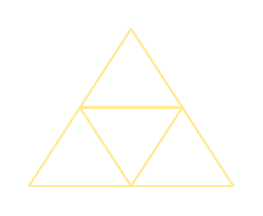
\begin{tikzpicture}
      \draw[color=acc, thick] (0, 0)--(1.3, -2);
      \draw[color=acc, thick] (0, 0)--(-1.3, -2);
      \draw[color=acc, thick] (1.3, -2)--(-1.3, -2);
      \draw[color=acc, thick] (0.65, -1)--(-0.65, -1);
      \draw[color=acc, thick] (0.65, -1)--(0, -2);
      \draw[color=acc, thick] (-0.65, -1)--(0, -2);
    \end{tikzpicture}
  \end{center}
  W kazdym z tych trojkatow odleglosc miedzy dwoma punktami nie moze przekraczac $2$. Podzielmy kazdy z nich znowu na 4 trojkaty rownoboczne o boku dlugosci 1:
  \begin{center}
    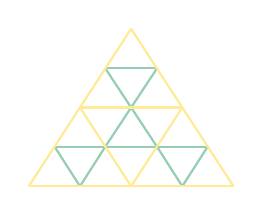
\begin{tikzpicture}
      \draw[color=emp, thick] (0.33, -0.5)--(-0.33, -0.5);
      \draw[color=emp, thick] (0.33, -0.5)--(0, -1);
      \draw[color=emp, thick] (-0.33, -0.5)--(0, -1);
      \draw[color=emp, thick] (-0.33, -1.5)--(0, -1);
      \draw[color=emp, thick] (0.33, -1.5)--(0, -1);
      \draw[color=emp, thick] (-0.97, -1.5)--(0.97, -1.5);
      \draw[color=emp, thick] (-0.97, -1.5)--(-0.65, -2);
      \draw[color=emp, thick] (-0.33, -1.5)--(-0.65, -2);
      \draw[color=emp, thick] (0.97, -1.5)--(0.65, -2);
      \draw[color=emp, thick] (0.33, -1.5)--(0.65, -2);
      \draw[color=acc, thick] (0, 0)--(1.3, -2);
      \draw[color=acc, thick] (0, 0)--(-1.3, -2);
      \draw[color=acc, thick] (1.3, -2)--(-1.3, -2);
      \draw[color=acc, thick] (0.65, -1)--(-0.65, -1);
      \draw[color=acc, thick] (0.65, -1)--(0, -2);
      \draw[color=acc, thick] (-0.65, -1)--(0, -2);
    \end{tikzpicture}
  \end{center}
  Dostajemy 16 trojkatow, w srodku ktorych odleglosci nie przekraczaja 1. Rozmieszczajac 17 punktow mamy pewnosc, ze co najmniej dwa z nich beda w tym samym trojkacie, wiec odleglosc miedzy nimi nie przekroczy 1.
\subsection*{\color{tit}ZAD 12. W kwadracie o boku 1 danych jest $2n+1$ punkotw, z ktorych zadne trzy nie sa wspolliniowe. Udowodnic, ze pewne trzy punkty tworza trojkat o polu $\leq\frac1{2n}$.}
  Dla dowolnego $n$ podzielmy kwadrat na $2n$ przystajacych trojkatow. Wowczas, sposrod $2n+1$ punktow co najmniej dwa musza lezec w tym samym trojkacie. 
\subsection*{\color{tit}ZAD 13. Na plaszczyznie danych jest piec punktow kratowych (o obu wspolrzednych calkowitych). Wykazac, ze srodek jednego z odcinkow laczacych te punkty tez jest kratowy.}
  Mamy 2 wspolrzedne, wiec uklad parzystych i nieparzystych wspolrzednych mozna wybrac na 4 sposoby. Jest 5 punktow, wiec co najmniej dwa z nich maja ten sam uklad, wiec ich suma bedzie miala obie wspolrzedne parzyste, a wiec srodek takiego odcinka ma wspolrzede calkowite.
\subsection*{\color{tit}ZAD 14. Udowodnic, ze dla kazdej liczby niewymiernej $\alpha$ istnieja ciagi liczb calkowitych $p_n, q_n,$ takie, ze $q_n\to\infty$ oraz}
$$\color{tit}|\alpha-\frac{p_n}{q_n}|<\frac1{q_n^2}$$
\subsection*{dla kazdego $n$.}
\subsection*{Wskazowka: Dla ustalonej liczby naturalnej $N$ rozpatrzyc ciag $n\alpha-[n\alpha]$ dla $n=0, 1, ...N$.}
\subsection*{ZAD 15. Udowodnic, ze dla danej liczby pierwszej $p>2$ istnieja liczby naturalne $x, y$, takie, ze liczba $1+x^2+y^2$ jest podzielna przez $p$.}
\subsection*{ZAD 16. Kazdy wierzcholek jedenastokata foremnego pomalowano na jeden z czterech kolorow. Udowodnij, ze mozna wybrac piec kolejnych wierzcholkow, pomalowanych co onajwyzej trzema kolorami.}
  Jesli bedziemy malowac na przemian kolorami, mozemy dojsc az do 8 wierzcholka i zostanie nam do pomalowania ostatnie 3, z ktorych dwa beda mialy ten sam kolor co dwa pomalowane na samym poczatku.\\
  11 wierzcholkow mozemy pogrupowac w dwie 4 czowrki, ktore pomalujemy roznymi kolorami i zostaje nam 3 luzne elementy. Poniewaz ustawiamy je "na kole", to 2 z luznych elementow beda lezaly obok siebie. Pomalujmy je na dwa rozne kolory, ktore sa rozne od kolorow wierzcholkow, przy ktorych leza. Niech maja te same kolory, co wierzcholki oddalone od nich o 1:
  \begin{center}
    
\begin{tikzpicture}
      \draw[color=def, fill=def, thick] (0, 0) circle (0.1);
      \draw[color=acc, fill=acc, thick] (0.5, 0) circle (0.1);
      \draw[color=emp, fill=emp, thick] (1, 0) circle (0.1);
      \draw[color=tit, fill=tit, thick] (1.5, 0) circle (0.1);
      \draw[color=emp, thick] (2, 0) circle (0.1);
      \draw[color=acc, thick] (2.5, 0) circle (0.1);
      \draw[color=def, fill=def, thick] (3, 0) circle (0.1);
      \draw[color=acc, fill=acc, thick] (3.5, 0) circle (0.1);
      \draw[color=emp, fill=emp, thick] (4, 0) circle (0.1);
      \draw[color=tit, fill=tit, thick] (4.5, 0) circle (0.1);
    \end{tikzpicture}
  \end{center}
  lub o 2:
  \begin{center}
    
\begin{tikzpicture}
      \draw[color=def, fill=def, thick] (0, 0) circle (0.1);
      \draw[color=acc, fill=acc, thick] (0.5, 0) circle (0.1);
      \draw[color=emp, fill=emp, thick] (1, 0) circle (0.1);
      \draw[color=tit, fill=tit, thick] (1.5, 0) circle (0.1);
      \draw[color=acc, thick] (2, 0) circle (0.1);
      \draw[color=emp, thick] (2.5, 0) circle (0.1);
      \draw[color=def, fill=def, thick] (3, 0) circle (0.1);
      \draw[color=acc, fill=acc, thick] (3.5, 0) circle (0.1);
      \draw[color=emp, fill=emp, thick] (4, 0) circle (0.1);
      \draw[color=tit, fill=tit, thick] (4.5, 0) circle (0.1);
    \end{tikzpicture}
  \end{center}
  W ten sposob mozemy zawsze znalezc 5 wierzcholkow, ktore sa pomalowane na co najwyzej 3 kolory.
\subsection*{ZAD 17. Kazdy punkt okregu pomalowano na jeden z dwoch kolorow. Wykaz, ze istnieje trojkat rownoramienny wpisany w ten okrag, o wszystkich trzech wierzcholkach jednego koloru.}
  Wybierzmy sieczna tego okregu, ktora nie jest srednica i ktorej oba konce maja ten sam kolor.
  \begin{center}
    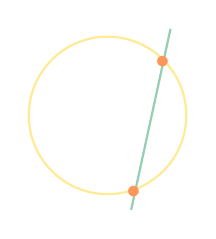
\begin{tikzpicture}
      \draw[color=acc, thick] (0, 1) circle (1);
      \draw[color=emp, thick] (0.3, -0.2)--(0.8, 2.1);
      \node(a) at (0.7, 1.67) {\color{def}$\bullet$};
      \node(b) at (0.33, 0.02) {\color{def}$\bullet$};
    \end{tikzpicture}
  \end{center}
  Narysujmy jej symetralna:
  \begin{center}
    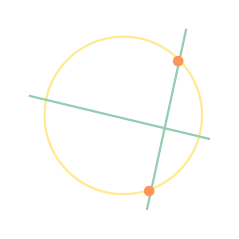
\begin{tikzpicture}
      \draw[color=acc, thick] (0, 1) circle (1);
      \draw[color=emp, thick] (0.3, -0.2)--(0.8, 2.1);
      \draw[color=emp, thick] (1.1, 0.7)--(-1.2, 1.25);
      \node(a) at (0.7, 1.67) {\color{def}$\bullet$};
      \node(b) at (0.33, 0.02) {\color{def}$\bullet$};
    \end{tikzpicture}
  \end{center}
  Jesli choc jeden z jej koncow jest tego samego koloru co konce poprzedniego odcinka, znalezlismy trojkat rownoramienny. W przeciwnym wypadku narysujmy symetralna tego wierzcholka:
  \begin{center}
    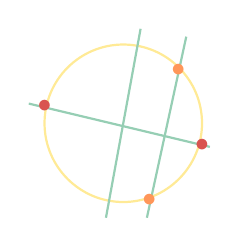
\begin{tikzpicture}
      \draw[color=acc, thick] (0, 1) circle (1);
      \draw[color=emp, thick] (0.3, -0.2)--(0.8, 2.1);
      \draw[color=emp, thick] (1.1, 0.7)--(-1.2, 1.25);
      \node(a) at (0.7, 1.67) {\color{def}$\bullet$};
      \node(b) at (0.33, 0.02) {\color{def}$\bullet$};
      \node(c) at (-1, 1.21) {\color{tit}$\bullet$};
      \node(d) at (1, 0.72) {\color{tit}$\bullet$};
      \draw[color=emp, thick] (-0.22, -0.2)--(0.22, 2.2);
    \end{tikzpicture}
  \end{center}
  Jesli oba konce tego wierzcholka maja inny kolor niz konce wierzcholka do nich rownoleglego, otrzymujemy trapez rownoramienny:
  \begin{center}
    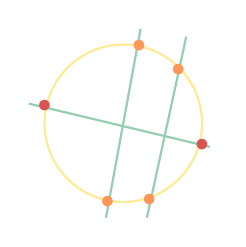
\begin{tikzpicture}
      \draw[color=acc, thick] (0, 1) circle (1);
      \draw[color=emp, thick] (0.3, -0.2)--(0.8, 2.1);
      \draw[color=emp, thick] (1.1, 0.7)--(-1.2, 1.25);
      \node(a) at (0.7, 1.67) {\color{def}$\bullet$};
      \node(b) at (0.33, 0.02) {\color{def}$\bullet$};
      \node(c) at (-1, 1.21) {\color{tit}$\bullet$};
      \node(d) at (1, 0.72) {\color{tit}$\bullet$};
      \draw[color=emp, thick] (-0.22, -0.2)--(0.22, 2.2);
      \node (e) at (-0.2, 0) {\color{def}$\bullet$};
      \node (f) at (0.2, 1.98) {\color{def}$\bullet$};
    \end{tikzpicture}
  \end{center}
  Teraz wystarczy znalezc punkty przeciecia symatralnych jego ramion z okregiem.
  \begin{center}
    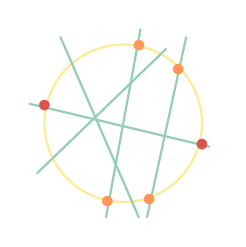
\begin{tikzpicture}
      \draw[color=acc, thick] (0, 1) circle (1);
      \draw[color=emp, thick] (0.3, -0.2)--(0.8, 2.1);
      \draw[color=emp, thick] (1.1, 0.7)--(-1.2, 1.25);
      \node(a) at (0.7, 1.67) {\color{def}$\bullet$};
      \node(b) at (0.33, 0.02) {\color{def}$\bullet$};
      \node(c) at (-1, 1.21) {\color{tit}$\bullet$};
      \node(d) at (1, 0.72) {\color{tit}$\bullet$};
      \draw[color=emp, thick] (-0.22, -0.2)--(0.22, 2.2);
      \node (e) at (-0.2, 0) {\color{def}$\bullet$};
      \node (f) at (0.2, 1.98) {\color{def}$\bullet$};
      \draw[color=emp, thick] (0.55, 1.95)--(-1.1, 0.36);
      \draw[color=emp, thick] (0.2, -0.20)--(-0.8, 2.1);
    \end{tikzpicture}
  \end{center}
  Jesli jeden z tych koncow jest tego samego koloru co ramie trapezu, mamy trojkat rownoramienny. W przeciwnym wypadku laczymy dwa konce i jeden z koncow symetralnej pierwszego narysowanego odcinka:
  \begin{center}
    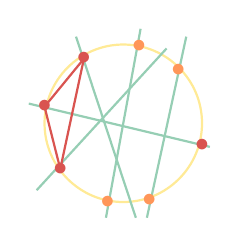
\begin{tikzpicture}
      \draw[color=acc, thick] (0, 1) circle (1);
      \draw[color=emp, thick] (0.3, -0.2)--(0.8, 2.1);
      \draw[color=emp, thick] (1.1, 0.7)--(-1.2, 1.25);
      \node(a) at (0.7, 1.67) {\color{def}$\bullet$};
      \node(b) at (0.33, 0.02) {\color{def}$\bullet$};
      \node(c) at (-1, 1.21) {\color{tit}$\bullet$};
      \node(d) at (1, 0.72) {\color{tit}$\bullet$};
      \draw[color=emp, thick] (-0.22, -0.2)--(0.22, 2.2);
      \node (e) at (-0.2, 0) {\color{def}$\bullet$};
      \node (f) at (0.2, 1.98) {\color{def}$\bullet$};
      \draw[color=emp, thick] (0.55, 1.95)--(-1.1, 0.15);
      \draw[color=emp, thick] (0.16, -0.20)--(-0.6, 2.1);
      \node(g) at (-0.50, 1.82) {\color{tit}$\bullet$};
      \node(h) at (-0.8, 0.42) {\color{tit}$\bullet$};
      \draw[color=tit, thick] (-0.50, 1.82)--(-1, 1.21);
      \draw[color=tit, thick] (-0.50, 1.82)--(-0.8, 0.42);
      \draw[color=tit, thick] (-0.8, 0.42)--(-1, 1.21);
    \end{tikzpicture}
  \end{center}
  \begin{center}
    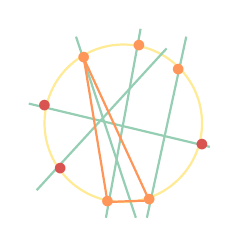
\begin{tikzpicture}
      \draw[color=acc, thick] (0, 1) circle (1);
      \draw[color=emp, thick] (0.3, -0.2)--(0.8, 2.1);
      \draw[color=emp, thick] (1.1, 0.7)--(-1.2, 1.25);
      \node(a) at (0.7, 1.67) {\color{def}$\bullet$};
      \node(b) at (0.33, 0.02) {\color{def}$\bullet$};
      \node(c) at (-1, 1.21) {\color{tit}$\bullet$};
      \node(d) at (1, 0.72) {\color{tit}$\bullet$};
      \draw[color=emp, thick] (-0.22, -0.2)--(0.22, 2.2);
      \node (e) at (-0.2, 0) {\color{def}$\bullet$};
      \node (f) at (0.2, 1.98) {\color{def}$\bullet$};
      \draw[color=emp, thick] (0.55, 1.95)--(-1.1, 0.15);
      \draw[color=emp, thick] (0.16, -0.20)--(-0.6, 2.1);
      \node(g) at (-0.50, 1.82) {\color{def}$\bullet$};
      \node(h) at (-0.8, 0.42) {\color{tit}$\bullet$};
      \draw[color=def, thick] (-0.50, 1.82)--(-0.2, 0);
      \draw[color=def, thick] (-0.50, 1.82)--(0.33, 0.02);
      \draw[color=def, thick] (-0.2, 0)--(0.33, 0.02);
    \end{tikzpicture}
  \end{center}
\subsection*{ZAD 18. Na plaszczyznie danych jest 6 punktow, z ktorych zadne trzy nie sa wspolliniowe. W kazdym trojkacie wyznaczonym przez pewna trojke tych punktow najkrotszy bok malujemy na zolto. Udowodnij, ze istnieje trojkat o wszystkich bokach zoltych.}
  Mamy 6 punktow, ktore mozemy polaczyc w odcinki na
  $${6\choose2}=15$$
  roznych sposobow. Z tych 15 odcinkow mozemy ulozyc 5 roznych trojkatow, w ktorych zaznaczymy 5 bokow na zolto. Poniewaz kazdy odcinek wykorzystalismy tylko jeden raz, zaden zolty bok nie zostal pomalowany dwa razy - mozemy teraz wybrac trzy dowolne zolte boki i stworzyc z nich trojkat o wszystkich bokach zoltych.
\end{document}